\documentclass[11pt,a4paper]{report}

\usepackage{graphicx}
\graphicspath{ {images/} }

\author{Catherine Vlasov}
\title{3rd Year Project Report}
\date{May 2018}

\begin{document}

\makeatletter
	\begin{titlepage}
		\vspace*{\fill}
		\begin{center}
			{\huge \bfseries \@title }
			\\[4ex]
			{\LARGE  \@author}
			\\[2ex]
			{\large \@date}
			\\[50ex]
			
\includegraphics[width=30mm]{oxlogo.png}
		\end{center}
		\vspace*{\fill}
	\end{titlepage}
\makeatother

\begin{abstract}
This is my abstract
\end{abstract}

\tableofcontents


%-----------------------
\chapter{Introduction}


%-----------------------
\chapter{Background}


\section{Reinforcement Learning}


\section{Learning Algorithms}


\subsection{Monte Carlo Learning}

\label{sec:monteCarloPseudocode}




%-----------------------------------------
\chapter{Design \& Implementation}

This section describes the implementations of Tic-Tac-Toe and Chung Toi as well as the game-playing agents used in this project's experiments. The source code is not provided in this report, but is available upon request.


\section{Overview} % including a UML diagram

The project is built in a modular way, using an object-oriented style. All actions, agents, games, and states implement general interfaces, called \emph{Action}, \emph{Agent}, \emph{Game}, and \emph{State} respectively, that serve as Facades for the complex implementations.

The \emph{Game} interface has a method \emph{play()} that simulates a single game. This is where the agents are asked to choose actions, receive returns, and complete other tasks, depending on the specific game. Agents do not distinguish between different games and only use methods defined in the general interfaces, which means that the \emph{MonteCarloAgent} class, for example, can be used to play both Tic-Tac-Toe and Chung Toi. This modularity provides a nice separation of concerns that enables simpler testing and debugging.


\section{Agents}

As part of this project, two agents were implemented: \emph{RandomAgent} and \emph{MonteCarloAgent}. 

\emph{MonteCarloAgent} implements the $\epsilon$-soft on-policy Monte Carlo control algorithm. In its \emph{chooseAction(State s)} method, it chooses an action according to its policy for states it has encountered in previous games, and randomly otherwise. In its \emph{gameOver()}, method it calls two private helper methods \emph{policyEvaluation()} and \emph{policyImprovement()} that update $Q$ and $\pi$, respectively, as described in section \ref{sec:monteCarloPseudocode}. Hash maps are used to store $\pi$ and $Q$ for constant time access and insertion.

As its name suggests, \emph{RandomAgent} randomly selects an action from the list of available actions at any given state. In total, the logic for this agent is equivalent to one line of code and this agent is only used for training and benchmarking purposes.


\section{Tic-Tac-Toe}

The first game used in this project is Tic-Tac-Toe. It was chosen because it has a small state space (less than $3^9 = 19,683$ states) and it is a conceptually simple game that most people are familiar with.


\subsection{Rules}

Although this is a widely-known game, the rules are still included here for reference and clarity.

First, one of the two players is randomly selected to use \textbf{X} tokens (the other player uses \textbf{O} tokens). From now on, these players are referred to as the ``X-player'' and ``O-player'', respectively. The game then consists of the two players alternately placing their tokens in empty spaces on a 3x3 grid, starting with the X-player. Figure \ref{tic-tac-toe-grid-example} is an example of a possible state of the grid.

% Not sure if this is necessary
\begin{figure}[htbp]
	\begin{center}
		
\includegraphics[width=50mm]{tictactoe_grid_example.png}
		\caption{Example of a Tic-Tac-Toe grid\label{tic-tac-toe-grid-example}}
	\end{center}
\end{figure}

The game has three possible endings:

\begin{itemize}
	\item \textbf{X-player wins}: three \textbf{X} tokens form a horizontal, vertical, or diagonal row
	\item \textbf{O-player wins}: three \textbf{O} tokens form a horizontal, vertical, or diagonal row
	\item \textbf{Draw}: the grid is filled and neither player has won
\end{itemize}

In all Tic-Tac-Toe implementations described in Section \ref{sec:TicTacToeImplementation}, agents receive a return of 1 when they win, -1 when they lose, and 0 when the game ends in a draw or the game is not yet over.


\subsection{Implementation}
\label{sec:TicTacToeImplementation}

The aim of this project is to investigate the effect of eliminating a game's state symmetries on the Monte Carlo algorithm's learning rate and optimal learning parameters. In the game of Tic-Tac-Toe, a state can be symmetrical with up to seven other states as result of flipping it in the following ways:

\begin{itemize}
	\item horizontal axis
	\item vertical axis
	\item horizontal axis and then vertical axis
	\item major diagonal (i.e. top left to bottom right)
	\item major diagonal and then horizontal axis
	\item minor diagonal (i.e. top right to bottom left)
	\item minor diagonal and then horizontal axis
\end{itemize}

Of course, for some states, the result of some of these flips are the same, which is why a state might have strictly less than seven other symmetrical states.

With this goal in mind, Tic-Tac-Toe was implemented in three ways:

\begin{itemize}

	\item \textbf{``Normal''}:
This version does not break any symmetry and was used as a baseline.

	\item \textbf{``Limited Actions''}:
This version breaks the symmetry between states by limiting the actions available from each state such that no two actions result in symmetrical states.

	\item \textbf{``Symmetric Equality''}: 
This version breaks the symmetry between states by considering two objects representing states to be ``equal'' if they are symmetrical.

\end{itemize}

An interesting result of the Limited Actions implementation is that it slightly alters the way the game is played. Suppose a \emph{RandomAgent} is asked to select a move from the game's initial state (i.e. empty grid). In the Normal implementation, there are nine possible actions: putting an \textbf{X} token in one of the nine grid cells. In the Limited Actions implementation, there are only three possible actions: putting an \textbf{X} token in a corner, in the middle of the grid, and in the middle of one of the sides. To give a specific example of how this changes the game, notice that the probability of the agent choosing the action that involves placing their token in the middle of the grid is $\frac{1}{9}$ in the Normal implementation and $\frac{1}{3}$ in the Limited Actions implementation. Thus, the agent will end up choosing this action three times as frequently in the latter version. However, this effect is ignored for the purposes of this project because in the limit of infinitely many games, the \emph{MonteCarloAgent} will encounter all states and choose all possible moves an equal number of times, thus computing an accurate expected return for each action.

Implementing the desired behaviour for the Symmetric Equality version was not as simple as initially expected. Overriding the \emph{equals()} method inherited from Java's \emph{Object} class was straightforward. However, overriding the inherited \emph{hashCode()} method was tricky.

A Java \emph{HashMap} places key-value mappings in buckets depending on the value returned by calling \emph{hashCode()} on the keys. Thus, if two keys have different hash codes, then they are placed in two different buckets, even if they are ``equal'' according to both of their \emph{equals()} methods. So, two ``equal'' keys (and their respective values) can both end up being stored in a hash map at the same time if they have different hash codes. This is why it was crucial for the \emph{hashCode()} method in \emph{TicTacToeStateWithSymmetricEquality} to produce exactly the same result for symmetrical states. After considering a few solutions, this behaviour was implemented by internally converting each state to a canonical form in such a way that symmetrical states have the same canonical form. Each state's canonical form is used to compute the state's hash code, which results in all symmetrical states having the same hash code, as required.

The idea behind the Limited Actions implementation is that it is expected to speed up the \emph{MonteCarloAgent}'s learning since only a fraction of the states will be reachable. Thus, after a fixed number of games, each possible state will be encountered more often than in the Normal implementation and so the expected return for each state will be more accurate. On the other hand, the Symmetric Equality implementation is expected speed up learning by allowing the \emph{MonteCarloAgent} to combine its learning from symmetric states therefore increasing the accuracy of its expected returns. In both cases, the agent's policy and action-value function will be smaller, which reduces the agent's memory requirements.


\section{Chung Toi}

The second game used is in the project is Chung Toi,  a more complex version of Tic-Tac-Toe that has been studied in the context of reinforcement learning before. Its state space is larger than that of Tic-Tac-Toe (i.e. less than $5^9 = 1,953,125$ states) which leads to interesting results.


\subsection{Rules}

The main idea behind Chung Toi is the same as that behind Tic-Tac-Toe in the sense that the game is played on a 3x3 grid and each player's goal is to get three of their pieces in a row. However, that is the entire extent of their overlap. Although the two games may seem similar, finding a good strategy for Chung Toi is not at all intuitive, unlike in Tic-Tac-Toe.

Before the game begins, one of the two players is randomly selected to use red tokens (the other player uses white tokens). From now on, these players are referred to as the ``red player'' and ``white player'', respectively. Each player has three tokens at their disposal and each token can be used in two possible orientations, as shown in Figure \ref{chung-toi-tokens}.

\begin{figure}[htbp]
	\begin{center}
		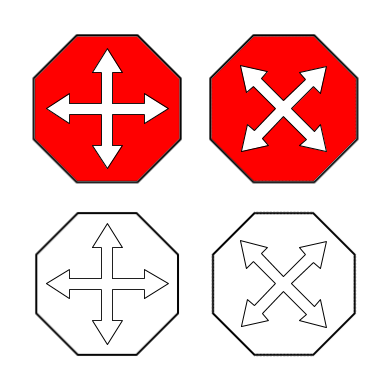
\includegraphics[width=40mm]{chung_toi_tokens.png}
		\caption[Chung Toi tokens]{Red and white Chung Toi tokens in both possible orientations}\label{chung-toi-tokens}
	\end{center}
\end{figure}

The game consists of the players alternately making a move, starting with the red player. Throughout the game, the red player can only move red tokens and the white player can only move white tokens. The game has two phases and both players start in Phase 1. Once a player places all three of their tokens, that player proceeds to Phase 2. The following actions are available in each phase:

\begin{itemize}

	\item \textbf{Phase 1}
		\begin{itemize}
			\item Place a token (in either orientation) in an empty grid cell
			\item Pass
		\end{itemize}

	\item \textbf{Phase 2}
		\begin{itemize}
			\item Slide a token on the grid in the direction of any of the arrows on that token. When the token reaches the final cell, it can be rotated (to switch its orientation) if the player chooses to do so. \emph{(Note: all grid cells in the path from the original cell to the final cell must be empty, meaning that the token cannot ``jump'' over other tokens)}
			\item Rotate one token (to switch its orientation)
			\item Pass
		\end{itemize}

\end{itemize}

At any point in the game, if both players pass, one right after the other, the game ends and is declared a draw. Otherwise, the game continues until one of the players makes their tokens form a horizontal, vertical, or diagonal row and that player is declared the winner. The orientation of the three tokens in the row does not matter.

Figure \ref{chung-toi-grid-example} is an example of a possible state of the grid.

\begin{figure}[htbp]
	\begin{center}
		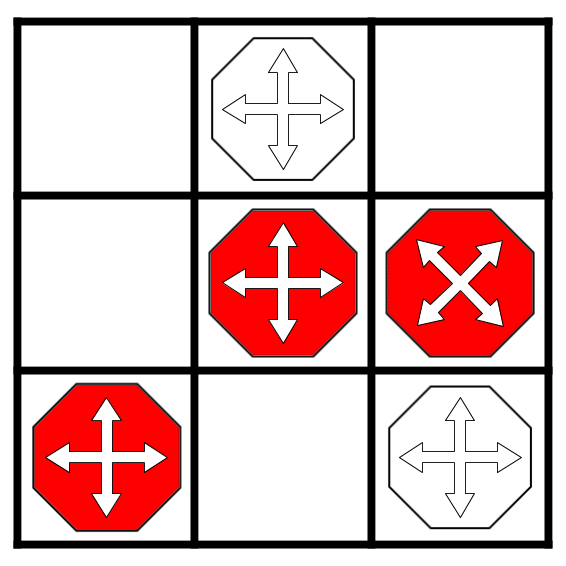
\includegraphics[width=50mm]{chung_toi_grid_example.png}
		\caption{Example of a Chung Toi grid\label{chung-toi-grid-example}}
	\end{center}
\end{figure}


\subsection{Implementation}

The role of Chung Toi in this project was to learn more about the effect of the Monte Carlo learning parameter $\epsilon$ on an agent's learning rate and winning rate. Chung Toi has roughly 100 times more states than Tic-Tac-Toe, which is expected to have an effect on the optimal value of $\epsilon$ and therefore \emph{MonteCarloAgent}'s learning rate.

Chung Toi has the same axes of symmetry as Tic-Tac-Toe, so similar results would be expected from a Chung Toi implementation that breaks symmetries. For this reason, such an implementation was not developed to reduce redundancy and instead only a normal implementation with all symmetrical states present was developed.


%------------------
\chapter{Results}


\section{Overview}


\section{Monte Carlo Learning Parameter}
% - Tic-Tac-Toe win rate graph for each value of alpha from 0.01 to 0.99
% - zoomed in graph for the region around global max. with more games per value
% - same graphs for both implementations of symmetry-breaking
% - analysis


\section{Policies} % ???
% - pick interesting examples and plot the policies vs. number of games ???


\section{Time}
% - discussion of time complexity


\section{Win/Learning Rate}
% - plot all three Tic-Tac-Toe types on the same graph



%-------------------
\chapter{Analysis} % or Discussion



%-----------------------
\chapter{Conclusion}


\section{Future Work}


\section{Personal Reflections}

This has been a really great learning experience, not only in terms of discovering the field of reinforcement learning and its applications, but also in terms of gaining experience with building up a large, complex programming project from scratch using a variety of technical tools.

When I was in high school, I designed and implemented the classic board game Nine Men’s Morris where a user plays against an algorithm I wrote. My plan for the project was to ask my friends and family to play my game and to store the moves made in each game so that I could build up a database of sequences of moves and outcomes of the game. I hoped to somehow compute which moves were the best and get my algorithm to learn which moves made winning the most likely. Little did I know, I wanted to invent RL from scratch – unaware of its existence or of the amount of research in the field. Several years later, I am delighted to have had the chance to work on a similar project, but this time on a deeper level using well-known computational algorithms.

When I started working on this project, I decided to treat it as an opportunity to develop many skills that are critical for a career in software engineering:

\begin{itemize}
	\item Writing clean, maintainable, well-documented code
	\item Designing and implementing tests for my code
	\item Using a build tool to manage dependencies between packages in my project as well as with external libraries
	\item Using version control effectively
\end{itemize}

I tested the methods in my API using a unit-testing framework for Java called JUnit. I also used a testing framework for Java called Mockito – this allowed me to verify the behaviour of objects with external dependencies by creating “mock objects” for theses dependencies, which mimic real objects but do so in a particular way that I can specify.

In order to save my experiment results in a format that would facilitate the creation of graphs, I used opencsv, a CSV parser library for Java.

To manage my project’s dependencies, I used a build tool developed by Google called Bazel and I used Git for version control.

Overall, I really enjoyed learning about RL algorithms and exploring their applications and success rates, all while developing strong programming skills that will help me throughout my career.


%--------------------------------
\chapter{Acknowledgements}

Thanks for reading.


\end{document}
